% ##################################################################################################################
\chapter{Zürich}
\label{ch:zhscenario}
\hfill \textbf{Author:} Andreas Horni

\editdone{This text has undergone the professional edit. Please no grammatical changes anymore! They are most-probably wrong.}

% ##################################################################################################################
The \gls{matsim} team frequently uses the Zürich scenario, based on the Switzerland scenario described above. The Zürich scenario, however, was more detailed; it was enhanced by data available only for the smaller region; \eg traffic light data or freight demand data was only included for Zürich city and the canton. It is under continuous development, calibration and validation and has been applied in numerous projects, serving as a real-world research example.   

\citet{HorniEtAl_TechRep_IVT_2011_a} provided a technical overview of the first scenario branch; \citet[][]{BalmerEtAl_ResRep_bdktzrh_2009} described its generation for the ``Westumfahrung'' project . 

The study area was delineated by a circle, with a 30\,kilometer radius around Bellevue, a central and prominent Zürich location. This delineation led to two versions,  the \emph{Zürich diluted scenario} and the \emph{Zürich cut scenario}. For the first, all agents crossing the study area during the simulated day were considered (Figure~\ref{fig:zurichScenario}), resulting in almost two million agents. For the second, only agents remaining in this area the whole day were modeled. The \emph{Zürich cut scenario} was employed as an experiment in \citet[][]{Hackney_PhDThesis_2009}, but using the \emph{Zürich diluted scenario} for production runs is preferable.

Demand was taken directly from the Swiss model; freight traffic was also added to the Zürich scenario, as follows. Canton Zürich raw freight traffic data was taken from the \gls{kvmzh}, provided by \citet{AMV_Webpage_2011} and documented in \citet[][]{GottardiBuergler_SV_1999}. Zonal level matrices were disaggregated to single \gls{matsim} plans \citep[][]{ShahM_TechRep_IVT_2010}. Matrices for small delivery and heavy trucks were combined into one activity called \emph{freight}. An additional 180\,000 agents were generated for the Zürich region.

For the diluted Zürich scenario, all Swiss facilities, as described above, were used as activity locations. For the diluted scenario, the networks were not thinned out. For  public transport simulation, network and transport schedules were derived from the \gls{kvmzh}. Walk and bike modes were ``\gls{teleported}''. 

Calibration was mainly done for modal split and distance distributions and utility function values set accordingly.

For validation, count data on city level, cantonal level and national level \citep[][]{ASTRA_Webpage_2006} were available from various sources, resulting in 123\,links measured for the Zürich inner city, delineated by a 12\,kilometer radius around Bellevue. The reduced count analysis radius was applied to reduce boundary effects resulting from demand reduction outside the 30\,kilometer radius study area. An average working day (Monday to Thursday, excluding public holidays) was used for comparison in current scenarios.

Some traffic signal data was available for Zürich city \citep[][]{STAPOZH-DAV_unpub_gtZH_2008}; this was integrated for the Westumfahrung project.
%
\createfigure%
{The diluted Zürich scenario}%
{The diluted Zürich scenario}%
{\label{fig:zurichScenario}}%
{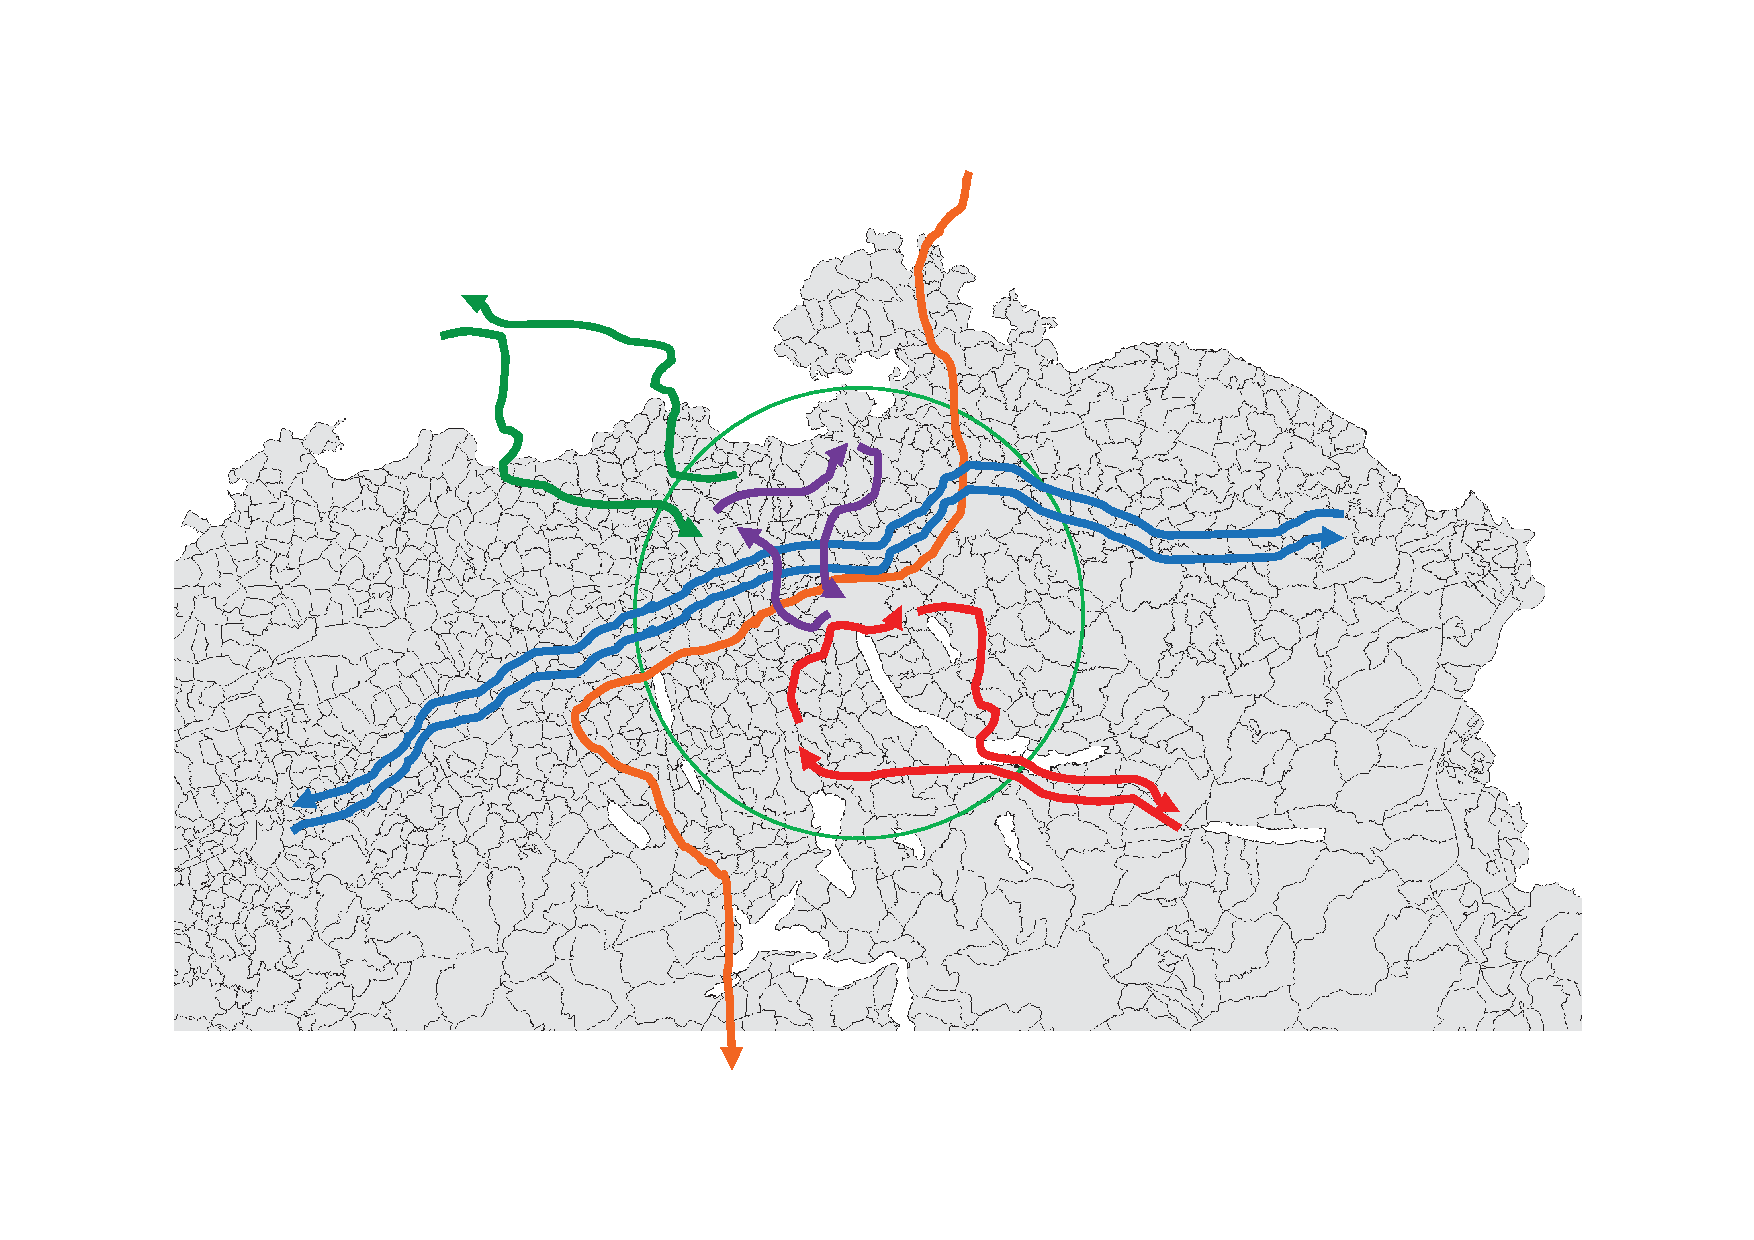
\includegraphics[width=0.99\textwidth, angle=0]{scenarios/figures/zh.pdf}}%
{}

% ##################################################################################################################
